\chapter{Resultados}
\label{cap:resultados}

La figura~\ref{fig:curvas} muestra varias curvas calculadas con pgfplots.

\begin{figure}[h]
  \centering
  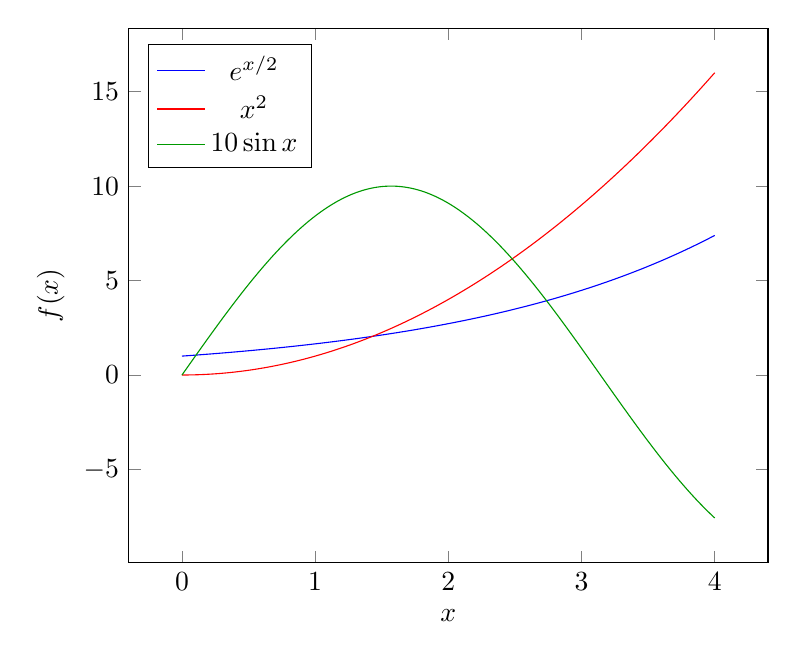
\begin{tikzpicture}
    \begin{axis}[width=0.8\textwidth, xlabel={$x$}, ylabel={$f(x)$}, legend pos=north west, samples=200]
      \addplot[blue, domain=0:4] {exp(x/2)};
      \addplot[red, domain=0:4] {x^2};
      \addplot[green!60!black, domain=0:4] {10*sin(deg(x))};
      \legend{$e^{x/2}$, $x^2$, $10\sin x$}
    \end{axis}
  \end{tikzpicture}
  \caption{Curvas de ejemplo.}
  \label{fig:curvas}
\end{figure}

\section{Análisis}
\lipsum[25-34]

\begin{figure}[h]
  \centering
  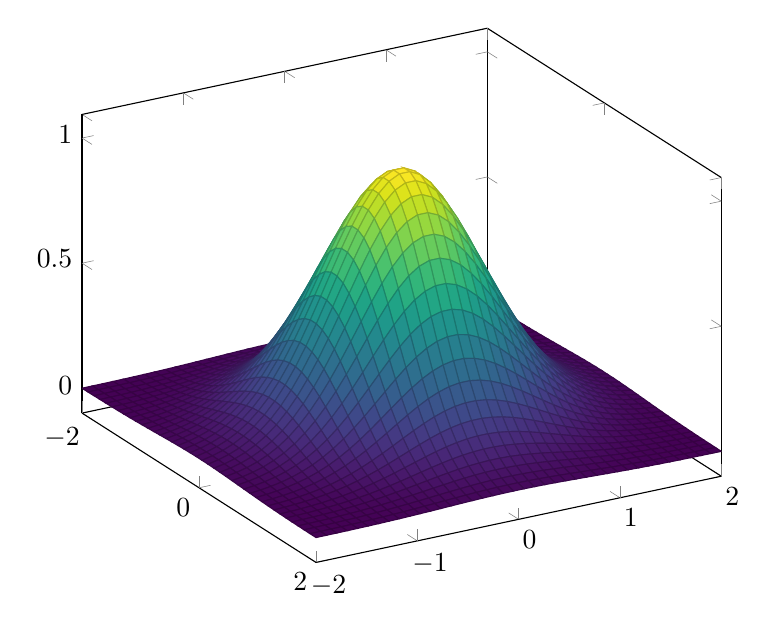
\begin{tikzpicture}
    \begin{axis}[width=0.8\textwidth, view={60}{30}, colormap/viridis]
      \addplot3[surf, domain=-2:2, samples=40] {exp(-x^2-y^2)};
    \end{axis}
  \end{tikzpicture}
  \caption{Superficie gaussiana.}
\end{figure}
